\section{Aufgabe 1 Typische Verzeichnisstrukturen}
	\begin{itemize}
		\item Geben Sie die typische Verzeichnisstruktur einer aktuellen Linuxdistribution an. Was ist
		in den Verzeichnissen enthalten? Nennen Sie mindestens fünf Beispiele (wie /etc, /usr
		usw.). Finden Sie zusätzlich heraus, wo Log-Dateien gespeichert werden.
		Wo liegen ausgelagerte Inhalte des Hauptspeichers?

		textbf{Antwort}: Ubuntu Verzeichnissystem entspricht Filesystem Hierarchy Standard(FHS):
		\footnote{Quellen:
		\href{http://www.pcwelt.de/ratgeber/So_funktioniert_die_Linux-Ordnerstruktur-Everything_is_a_file-8772939.html}{www.pcwelt.de},
		\href{http://www.selflinux.org/selflinux/html/verzeichnisse_unter_linux01.html}{www.selflinux.org},
		\href{https://jankarres.de/2014/01/debian-linux-verzeichnisbaum-erklaert}{jankarres.de},
		\href{https://wiki.ubuntuusers.de/Verzeichnisstruktur}{wiki.ubuntuusers.de},
		}
		\begin{itemize}
			\item \textbf{/} - Wurzelverzeichnis für alle anderen Linux Verzeichnisse.
			 In der Regel entspricht dieses der Bootpartition (wenn nicht anders beim Installieren eingestellt),
			 deswegen enthält es symbolische Verknüpfungen für initrd.img und vmlinuz,
			 die im Ordner \textit{/boot} liegen
			 \item \textbf{/boot} - beinhaltet alle für den Systemstart(Booten) benötigten Dateien
			 solche wie z.B Kernel \footnote{
			 für Desktop \textit{vmlinuz-versionsnummer-generic},
			 für Server \textit{vmlinuz-versionsnummer-server},
			 für virtuelle Maschinen \textit{vmlinuz-versionsnummer-virtual}
			 }, initiale Ramdisk \footnote{
			 \textit{initrd.img-versionsnummer-generic}/-\textit{server}/-\textit{virtual}}
			 und das Programm für den Memorytest \textit{memtest86.bin}.
			 Außerdem enthält dieser Verzeichnis Ordner \textit{grub/} mit den Bootloader Dateien
			 und dem Ordner \textit{efi/} mit EFI-Programmen
			 Dieses Verzeichnis muss beim Systemstart vorhanden sein.
			\item \textbf{/bin} - Enthält ausführbare Dateien (Programme).
			Es handelt sich bei den Dateien um System-Tools(z.B s cp, echo, mkdir, rm), die von allen Benutzern
			genutzt werden( im Gegensatz zu \textit{/sbin}). - Dieser Ordner darf keine
			weiteren Verzeichnisse enthalten. Dieses Verzeichnis muss beim Systemstart vorhanden sein.
			\item \textbf{/dev} - Dieses Verzeichnis beinhaltet alle für den Zugriff
			auf die Geräte erforderliche Dateien (z.B. für  Festplatten, DVD-Laufwerke, Maus, Monitor).
			Hier werden z.B. Festplaten Partitionen eingebunden. Die Dateien werden als Schnittstellen
			für Hardware benutzt.
			(ausgenommen sind jene die mit hot-Plugin eingebunden werden, dafür gibt es den Ordner \textit{/udev})
			Diese Verzeichnis muss beim Systemstart vorhanden sein.
			\item \textbf{/etc} - steht für \textit{``editable text configuration''}.
			Hier liegen systemweit gültige Konfigurations- und Informationsdateien des Basissystems.
			Hier findet man solche Dateien wie z.B. \textit{fstab, hosts, lsb-release, blkid.tab}.
			Diese Konfigurationsdateien können von gleichnamigen Dateien im Homeverzeichnis überschrieben werden.
			Der Ordner enthält viele Verzeichnisse mit Konfigurationsdateien.
			Beispiele:
			\begin{itemize}
				\item \textit{/etc/opt}: Verzeichnisse und Konfigurationsdateien für Programme in /opt
				\item \textit{/etc/network}: Verzeichnisse und Konfigurationsdateien des Netzwerkes (Interfaces u.s.w.)
				\item \textit{/etc/init.d}: Enthält Start- und Stopskripte
				\item \textit{/etc/hosts} Einstellungen für IP-Adressen Auflösung
				\item \textit{/etc/ssh/} enthält SSH Konfigurationsdateien
				\item \textit{/etc/X11} Konfigurationen für grafische X-Window-Subsystem
			\end{itemize}
			Dieses Verzeichnis muss beim Systemstart vorhanden sein.
			\item \textbf{/home} - Dieses Verzeichnis enthält ein Home-Ordner jedes Benutzers
			(als Name wird der Benutzername übernommen). Hier speichern die Benutzer Persönliche Daten, Eigene Programme,
			und Konfigurationsdateien die nur für den konkreten Benutzer beim Einloggen verfügbar sind.
			Der User hat volle Schreib- und Leserechte für das eigene Homeverzeichnis.
			Dieser Ordner kann auf eine andere Partition verlegt werden.
			Dieses Verzeichnis muss nicht beim Systemstart vorhanden sein.
			\item \textbf{/lib},\textbf{/lib32},\textbf{/lib64}  - hier liegen wichtige dynamische Bibliotheken des Systems und Kernel-Modules,
			viele werden beim Systemstart benötigt. z.B:
			\begin{itemize}
				\item \textit{/lib/modules} - Kernelmodule
				\item \textit{/lib/udev}: Bibliotheken und Programme für udev
				\item \textit{/lib/linux}-restricted-modules: Speicherort für eingeschränkte Treiber (z.B. Grafikkarte)
			\end{itemize}
			\item \textbf{/lost+found} - Das Verzeichnis ist in ext2, ext3 und ext4 Dateisystemen vorhanden.
			Der Ordner beinhaltet Dateien auf der Festplatte,
			die in der Verzeichnisstruktur nicht mehr zugeordnet werden können (bei System-/Programmabstürze oder Hardware-Fehler).
			Bei einem normal funktionierenden System soll der Ordner leer bleiben.
			\item \textbf{/media} - Das Verzeichnis wird nur als Einhängepunkt für Wechseldatenträger
			(solche wie Disketten \textit{/media/floppy}, CD-/DVD-Laufwerke \textit{/media/cdrom},
			\textit{/media/dvd}, Zip-Disks \textit{media/zip}, externe USB-Festplatten).
			Das Verzeichnis muss auf der gleichen Partition mit dem Root-Verzeichnis liegen.
			\item \textbf{/mnt} - Der Verzeichnis wird als Einhängepunkt für temporär verfügbare Dateisysteme
			(z.B. eine Windows Partition um auf die dort gespeicherten Daten zuzugreifen). Theoretisch könnte man
			das Verzeichnis als Einhängepunkt für Wechseldatenträger nutzen, dies wiederspricht aber den
			FHS Standard.
			\item \textbf{/opt} - Dieser Ordner wird für die manuelle Installation von Programmen genutzt.
			Deas Verzeichnis ist optional und ist nicht für den Start des Systems notwendig.
			Deswegen kann er auch auf andere Partition verlagert werden.
			\item \textbf{/proc} - Das Verzeichnis beinhaltet Prozess- und Systeminformationen und stellt die Schnittstelle zum Kernel dar
			und ist im eigentlichen Sinne ein spezielles, virtuelles Dateisystem.
			z.B: Beispiele:\textit{version} - Kernelversion, \textit{swaps} Swapspeicherinformationen, \textit{cpuinfo}, \textit{interrupts}, usw.
			Außerden liegen hier Verzeichnisse mit Prozessnumer als Name, die Dateien zu Prozessinformationen enthalten, solche wie
			\textit{status} Prozessstatus, \textit{limits} Limits für Ressourcen Verbrauch.
			Dieser Ordner ist nicht FHS Standard aber standardmäßig in Linux Distribution vorhanden. Muss beim Systemstart vorhanden sein.
			\item \textbf{/root} - Das ist das Homeverzeichnis des Superusers (root).
			Hier hat nur der Superuser volle Schreib- und Leserechte.
			Dieser Ordner muss immer vorhanden sein.
			\item \textbf{/run} - Der Ordner wird für Dateien von laufenden Prozessen genutzt.
			Hier liegen die meisten PID-Files \textit{*.pid} (Process identifier).
			\item \textbf{/sbin } - Hier liegen system binaries, die für essentielle Aufgaben der Systemverwaltung
			notwendig sind. Diese Programme können nur vom Superuser ausgeführt werden.
			Der Ordner muss auf der Rootpartition immer vorhanden sein.
			\item \textbf{/srv }- Hier liegen Dateien für System-Dienste.
			Oft werden hier variable Dateien solche wie Logfiles oder Mails eines Webservers gespeichert,
			(in unserem Ubuntu 14.04 ist dieser Ordner leer).
			Das Verzeichnis ist optional und ist nicht in allen Linuxdistributionen vorhanden.
			\item \textbf{/sys} - Das Verzeichnis hat eine ähnliche Funktion wie \textit{/proc} und beinhaltet
 			hauptsächlich Kernelschnittstellen.
		  Der Ordner ist im FHS noch nicht spezifiziert.
			\item \textbf{/tmp} - Wird für temporäre Dateien von Programmen genutzt.
			Nach FHS standart wird dieser Ordner nach jedem Neustart bereinigt.
			Jeder Benutzer hat vollen Zugrif nur auf seine eigenen temporären Dateien.
			\item \textbf{/usr} - Diese Verzeichnisstruktur enthält die meisten Systemtools, Bibliotheken und installierten Programme.
			Hier werden Programme gespeichert die von Paketverwaltung installiert wurden.
			Es liegen folgende Unterordner vor:
			\begin{itemize}
				\item \textit{/usr/bin} - Hier werden Ausführbare Programme gespeichert
				\item \textit{/usr/include} - Hier befinden sich Header-Dateien, die man bei der C-Programmierung
				im Source-Code inkludiert.
				\item \textit{/usr/lib} - Weitere Programm-Bibliotheken
				\item \textit{/usr/local} - Der Ordner hat die gleiche Struktur wie \textit{/usr} selbst, und kann
				für manuell installierte Programme genutzt werden (wie /opt).
				\item \textit{/usr/sbin} - Hier liegen optionale Systemprogramme
				\item \textit{/usr/share} - Hier liegen sich nicht ändernde, architekturunabhängige Dateien.
				\item \textit{/usr/share/applications} - Hier findet man Programmstarter, die für Anwendungsmenüs genutzt werden
				\item \textit{/usr/share/man} - Beinhaltet Man-pages
			\end{itemize}
			\item \textbf{/var } - Wird zur Speicherung von veränderlichen Daten genutzt. Hier liegen nur Verzeichnisse,
			deren Inhalt regelmäßig verändert wird.
			z.B. in \textit{/var/log} In dem Ordner werden ständig Logdateien überschrieben und neu angelegt.


		\end{itemize}
\item Geben Sie die typische Ordnerstruktur von Microsoft Windows an. Nennen Sie analog
zur vorherigen Aufgabe einige beispielhafte Inhalte der jeweiligen Verzeichnisse (wie z.B,
\textit{C:\textbackslash Windows\textbackslash System32}).
\textbf{Antwort:} Windows Ordner: (Pfade/Bezeichnungen können je nach Betriebssystem abweichen)
\footnote{Quellen:
\href{https://technet.microsoft.com/en-us/library/bb457124.aspxEEAA}{www.technet.microsoft.com},
\href{https://de.wikipedia.org/wiki/Sonderverzeichnis}{www.wikipedia.org/wiki/Sonderverzeichnis},
\href{https://en.wikipedia.org/wiki/Program_Files}{www.wikipedia.org/wiki/Program\_Files},
}

\begin{itemize}
	\item \textbf{System32}:	\textit{C:\textbackslash Windows\textbackslash System32} -
	ist das Systemverzeichnis von Windows. Hier liegen für das System essentielle
	Daten, Programme und Bibliotheken

	Inhalte:
	\begin{itemize}
		\item \textit{C:\textbackslash Windows\textbackslash System32\textbackslash Configuration} - Konfigurationsdateien.
		\item \textit{C:\textbackslash Windows\textbackslash System32\textbackslash config} - Registry Dateien und Event logs.
		\item \textit{C:\textbackslash Windows\textbackslash System32\textbackslash de-DE} - hier liegen die Lokalisierungspakete für die deutsche Sprache
		\item \textit{C:\textbackslash Windows\textbackslash System32\textbackslash GroupPolicy} - administrative Templates und Scriptfiles (Gruppenrechte)
		\item \textit{C:\textbackslash Windows\textbackslash System32\textbackslash Microsoft} - Kryptographie Dateien (Verschlüsselung)
\end{itemize}
 \item \textbf{Program Files:}	 \textit{C:\textbackslash Program Files(x86)} -
	ist der standard Ordner von Microsoft indem Anwendungen gespeichert werden, die
	nicht zum Betriebssystem gehören. Jede Anwendung erhält zusätzlich ein Unterverzeichnis für
	ihre Ressourcen. Die Bezeichnung kann je nach Betriebssystem den Zusatz (x86) bzw. (x64) mit
	sich führen. Im Ordner \textit{Program Files(x86)} werden 32 Bit Anwendungen und im Ordner
	\textit{Program Files(x64)} 64 Bit Anwendungen standardmäßig gespeichert.

	Inhalte:
	\begin{itemize}
		\item \textit{C:\textbackslash Program Files\textbackslash Adobe}
		\item \textit{C:\textbackslash Program Files\textbackslash MSBuild}
		\item \textit{C:\textbackslash Program Files\textbackslash Microsoft.NET}
		\item \textit{C:\textbackslash Program Files\textbackslash Mozilla Firefox}
		\item \textit{C:\textbackslash Program Files\textbackslash Windows Media Player}
\end{itemize}
\item \textbf{Desktop:}	 \textit{C:\textbackslash Users\textbackslash Username\textbackslash Desktop} -
	existiert zum Einen als Sonderverzeichnis und zum Anderen als virtuelles Verzeichnis.
	Das Sonderverzeichnis enthält die Dateien, die auf dem Desktop des Benutzers gespiechert sind.
	Beim virtuellen Verzeichnis handelt es sich um den Windows-Desktop. Ein Sonderverzeichnis hat einen
	Bezug zu einem echten Verzeichnis auf dem Dateisystem.

	Inhalte:
	\begin{itemize}
	\item \textit{C:\textbackslash Username\textbackslash Desktop\textbackslash4.Semester}
	\item \textit{C:\textbackslash Username\textbackslash Desktop\textbackslash Urlaubsfotos}
	\item \textit{ C:\textbackslash Username\textbackslash Desktop\textbackslash BSPraktikum }
	\item \textit{ C:\textbackslash Username\textbackslash Desktop }
	\item \textit{ C:\textbackslash Username\textbackslash Desktop\textbackslash Softwareprojekt }
\end{itemize}

\item \textbf{Favoriten:}	\textit{C:\textbackslash Users\textbackslash sername\textbackslash Favorites} -
	Hier befinden sich die Favoriten des Benutzers. Links die im Browser als Favoriten
	hinterlegt sind. Favorisierte Dokumente und Verzeichnisse des Nutzers werden im Ordner \textit{Links}
	gepeichert. \textit{C:\textbackslash Users\textbackslash Username\textbackslash Links}

	Inhalte:
	\begin{itemize}
	\item \textit{C:\textbackslash Users\textbackslash Username\textbackslash Favorites\textbackslash Acer\textbackslash Acer.url}
	\item \textit{C:\textbackslash Users\textbackslash Username\textbackslash Favorites\textbackslash Acerv\textbackslash eBay.url}
\end{itemize}

\item 	\textbf{Eigene Dateien:} 	\textit{C:\textbackslash Users\textbackslash Username} -
Hier befinden sich die Dokumente/Verzeichnisse des Benutzers.

Inhalte:
	\begin{itemize}
	\item \textit{C:\textbackslash Users\textbackslash Username\textbackslash Pictures}
	\item \textit{C:\textbackslash Users\textbackslash Username\textbackslash Music}
	\item \textit{C:\textbackslash Users\textbackslash Username\textbackslash Videos}
	\item \textit{C:\textbackslash Users\textbackslash Username\textbackslash Favorites}
	\item \textit{C:\textbackslash Users\textbackslash Username\textbackslash Links}
	\end{itemize}
\end{itemize}
	\end{itemize}

	\subsection{Fazit}
	In der Linux Distribution werden Log Dateien nach FHS Standart im Verzeichnis \textit{/var/log} hinterlegt.
	In Linux werden Inhalte des Hauptspeichers auf eine spezielle swap-Partition ausgelagert. Wir können in
	\textit{/proc/swap} Dateien sehen, die in unserem konkreten Ubuntu-System die Inhalte auf \textit{/dev/sda4} auslagert.

	Bei Windows und Linux gibt es Verschiedene Standarte für Verzeichnis Struktur.

\newpage
\section{Aufgabe 2 Typische Verzeichnisstrukturen}
Bearbeiten Sie die folgenden Aufgaben und protokollieren Sie Ihr Vorgehen mithilfe der Vorlage.
Entwickeln Sie ein Programm myls, das den Inhalt von Verzeichnissen ausgibt. Die grundle-
gende Funktion ist in etwa vergleichbar mit dem Shell-Kommando ls.
\subsection{Vorbereitung}
Zur Testzwecken haben wir einen Test Ordner erstellt \textit{testDir}.
im Ordner haben wir einige Dateien und Verzeichnise angelegt(darunter ein symlink und versteckte Dateien):
\begin{lstlisting}
	cd testDir
	touch fileOwnerUserGroupUser
	touch fileOwnerUserGroupTest
 	touch file1
 	touch .hiddenFile
 	touch file.c
 	touch file.cpp
	touch file2.c
 	mkdir dir1
 	mkdir .dirHidden
	touch ausfuerbar
	ln -s fileOwnerUserGroupTest symLinkToFileOwnerUserGroupTest
\end{lstlisting}
wir legen auch eine test Gruppe an, um dn Ergebnis der \command{myls} mit Parametern -g und -o
sichtbar unt beser interpretierbarer zu machen, denn von uns erstellte Dateien haben als default
userid = 1000 und Gruppenid = 1000

\begin{lstlisting}
sudo addgroup test
Lege Gruppe test (GID 1001) an ...
Fertig.
\end{lstlisting}
nun haben wir eine Gruppe mit Id 1001

wir ändern die Gruppe von File fileOwnerUserGroupTest zu Gruppe mit Id 1001
\begin{lstlisting}
sudo chown -c :test fileOwnerUserGroupTest
\end{lstlisting}
File \textit{ausfuerbar} bird ausfürbar gemacht

\subsection{Durchführung}
\begin{itemize}
	\item Zuerst definieren wir die maximale länge für Pfad \command{\#define MAX_PATH 1024}
\item Wir definieren eine Variable die den aktuellen Pfad speichert \command{char path[MAX_PATH];}
	\item Der Name des auszulesenden Verzeichnisses soll dem Programm als Argument übergeben
 werden. Wird kein Verzeichnis angegeben, so wird das lokale Verzeichnis ausgegeben.

 \item Hierzu nutzen wir die Eingabeparameter der main-Methode.\newline
  \command{main(int argc, char *argv[])} Um Parameter annehmen zu können
 nutzen wir die Variable argc um die Anzahl der übergebenen Argumente
 zu zählen sowie das Array argv um die Argumente auslesen zu können.
\item Im nächsten Schritt prüfen wir die Anzahl der übergebenen
Argumente.
\newline
\command{if (argc > 1 && strncmp(argv[1],"-",1)!=0)}
\newline
Wurden Argumente übergeben so ist die Variable argc größer als 1.
Zusätzlich prüfen wir ob das erste übergebene Argument mit einem - anfängt
(mittels strncmp aus header string.h, es wird nur das erste Zeichen geprüft).
Dies würde bedeuten dass der User das listing aus dem lokalen Pfad ausführen
möchte da das - Zeichen das Zeichen für die Parameter ist.
Ist dies der Fall so wird der else-Teil ausgeführt. Dieser wird auch ausgeführt
wenn keine Argumente übergeben werden.
\command{getcwd(path, MAX_PATH);} Im else-Teil wird dann das aktuelle
Working Directory mittels getcwd ermittelt und dem Array path übergeben.
Wurde ein Pfad übergeben so betrachten wir den If Block.
\command{strcpy(path, argv[1]);} Hier überweisen wir dem path Array den vom
User übergebenen Pfad.
\item Danach bauen wir eine Abfrage ein ob ein übergebener Pfad mit einem
/ endet. Ist dies nicht der Fall so hängen wir eines an.
Hierzu ermitteln wir zunächst die Länge des Pfades:
\command{int len = strlen(path);}
Dann erzeugen wir einen Pointer der auf den letzten Index des Arrays
zeigt \command{const char *last = &path[len - 1];}
Nun prüfen wir ob dieses Zeichen ein / ist
\command{if (strcmp(last, ``/'') != 0)}
Ist dies nicht der Fall so hängen wir eins an.
\command{strcat(path,"/");}
Diese Methoden der String-Manipulation entstammen dem string.h Header.
\item Wir definieren eine Variable \command{int c;} wo wir eine einzige Option
aus der übergebenen Options Liste speichern
\item Um die Optionen für myls zu speichern und weiter auszuwerten legen wir drei Variablen an
\begin{itemize}
	\item \command{int aoption = 0} für Option -a (gültige Werte 0 oder 1)
	\item \command{int loption = 0;} für -l und g Option (gültige Werte 0, 1, 2)
	\item \command{int ooption = 0;} für -o Option (gültige Werte 0 oder 1)
\end{itemize}

\item Wir nutzen die Funktion \command{getopt(argc, argv, ``algo'')} aus dem Header \command{unistd.h},
die das Auslesen der Optionen aus dem Argument-string erleichtert. Als ersten und zweiten Argument
werden die Argumente die die main Methode erhält an \command{getopt()} übergeben,
das dritte Argument übergeben wir als String aus allen gültigen Argumenten,
nach denen durchgesucht wird.
Wenn es keine Argumente in \command{argv0} gibt, dann liefert die Methode den Wert -1 zurück.
\item Den Rückgabewert von \command{getopt} nutzen wir als Abbruch Bedingung für die while-Schleife

\command{while ((c = getopt(argc, argv, ``algo'')) != -1)}
\item In der while-Schleife prüfen wir mit switch-case welche Option ausgelesen wurde,
und ändern die Werte von den oben genannten Variablen: a-,l-,ooption.
Wird beispielsweise ein a gelesen so wird der zutreffende case ausgeführt
und das aoption Flag auf 1 gesetzt.
Bei einem gelesenen l wird die loption auf 1 gesetzt.
Wird ein g gesetzt so wird die loption auf 2 gesetzt, folglich erkennen wir
dass das längere Ausgabeformat aber ohne UserID gewünscht ist.
Wird ein o gesetzt so setzen wir die ooption auf 1. Zudem prüfen wir
ob das loption Flag bereits gesetzt wurde. Wurde beispielsweise nur ein
o als Parameter übergeben so müssen wir das loption Flag auf 1 setzen damit
wir wissen dass das längere Ausgabeformat gewünscht ist.
Die ooption sorgt dafür dass die GroupID ausgeblendet werden soll.
Kombinationen der Parameter sind somit möglich.
\item Danach rufen wir die Funktion \command{readPath(path, aoption, loption, ooption);}
auf. Wir übergeben hier den Pfad sowie die 3 Flags.

 \begin{lstlisting}
	 int main(int argc, char *argv[]) {
	if (argc > 1 && strncmp(argv[1],"-",1)!=0) {
		strcpy(path, argv[1]);
	} else {
		getcwd(path, MAX_PATH);
	}
	int len = strlen(path);
	const char *last = &path[len - 1];
	if (strcmp(last, "/") != 0) {
		strcat(path,"/");
	}
	printf("input path: %s", path);
	int c;
	int aoption = 0;
	int loption = 0;
	int ooption = 0;
	while ((c = getopt(argc, argv, "algo")) != -1) {
		switch (c) {
		case 'a':
			aoption = 1;
			break;
		case 'l':
			loption = 1;
			break;
		case 'g':
			loption = 2;
			break;
		case 'o':
			if(loption==0)
				loption=1;
			ooption = 1;
			break;
		}
	}

	readPath(path, aoption, loption, ooption);
	return 0;
}
 \end{lstlisting}
\item Um den Verzeichnis Inhalt und Informationen auszulesen definieren wir eine Funktion

\command{void *readPath(char *path, int aoption, int loption, int ooption)}

\item Die Funktion nimmt als erstes Argument den Verzeichnisnamen, deren Inhalt ausgelesen wird,
die 3 folgenden Argumente sind die FLags.
\item Um Ordner Information zu lesen nutzen wir die Bibliothek \command{dirent.h},
\item Wir legen uns eine Variable für den aufgelösten Pfad an, mit der
bereits definierten Größe des maximalen Pfades
\command{char resolved_path[MAX_PATH];}
Außerdem definieren wir eine Variable  \command{DIR *dir = NULL;},
die den Directory Stream beinhalten wird.

Um den Ordner Inhalt aus dem directory stream zu lesen,definieren wir eine Variable

\command{struct dirent *dptr = NULL;}

Und eine Char Variable die lediglich einen Punkt hält, die wir zum Vergleich
nutzen werden.
\command{char *dot = ``.'';}

\item Um den absoluten Pfad zu erhalten nutzen wir die Funktion
\newline
\command{realpath((char*)path, resolved_path)}
\newline
aus der Standartbibliothek,
als Parameter übergeben wir den vom Benutzer übergebenen Pfad \command{path}
und unsere Variable \command{resolved_path}, die das Ergebnis erhalten wird,
dabei casten wir die Variable \command{path} zu einem char pointer.
Die Funktion wird einen \command{NULL} pointer zurückliefern, falls beim Pfadname auflösen ein Fehler auftritt,
deswegen können wir das Ergebnis der Variable \command{realpath} in der If-Abfrage überprüfen,
und falls etwas mit dem Pfad nicht stimmt, kann die Funktion \command{readPath} ihre Arbeit abbrechen.
\item Wenn der Pfad erfolgreich aufgelöst wurde können wir weiter vorgehen.
\item Wir öffnen den directory stream mit der Funktion \command{opendir(resolved_path)},
die Funktion wird einen \command{NULL} Pointer zurückliefern wenn ein Fehler beim Öffnen auftritt.
Wir fragen dsd Resultat ebenfalls in der If-Abfrage ab, wenn der Ordner erfolgreich geöffnet wurde,
kann man weiter vorgehen, ansonsten muss die Funktion \command{readPath} ihr Arbeit abbrechen.

\command{if ((dir = opendir(resolved_path)))}

\item Nun kann man mit der While-Schleife durch die einzelnen Einträge im
directory stream iterieren,
dabei hilft uns die Variable \command{dptr}, die bei jeder Iteration auf
den nächsten Eintrag zeigt.
Um den nächsten Eintrag auszulesen, benutzen wir die Funktion \command{readdir(dir)},
die als Parameter einen directory stream annimmt

\command{while ((dptr = readdir(dir)))}

\item Innerhalb der while-Schleife prüfen wir ob das aoption Flag NICHT gesetzt ist
\command{if (!aoption)}

Wir schließen die Dateien die mit dem Namen \textit{.} beginnen aus,
indem wir den Namen des aktuellen Eintrags mit der Variable \command{dot} vergleichen.
Und wenn es sich um diese Dateien handelt, geht die while schleife
ohne weiteres Vorgehen zur nächsten Iteration.

\command{if (strncmp(dptr->d_name, dot, 1) == 0) continue;}

\item Ist das a-Flag also gesetzt so nehmen wir auch die Versteckten Dateien
mit.

\item Nun prüfen wir ob das l-Flag gesetzt wurde \command{if (loption!=0)}

Ist dies der Fall, so legen wir uns eine Struktur vom Typ stat an, wo
wir Dateiinformationen speichern können.
\command{struct stat lstruct;}

Die Methode \command{printlstruct(dptr->d_name,loption, ooption);} wird
später erklärt. Sie erhält als Eingabeparameter den aktuellen File-Namen, sowie
die l- und o-Flags.

\item Mittels \command{lstat(dptr->d_name, &lstruct)} lesen wir die Information von der aktuellen Datei aus
und Speichern diese in der vorher definierten \command{lstruct} Variable.
Dabei folgt die Funktion im Gegensatz zur Funktion \command{stat()} nicht dem symbolic link,
sondern es wird die Information über den Link selbst ausgelesen und nicht über die referenzierte Datei.
Wenn die Information erfolgreich ausgelesen wurde, liefert die funktion den Wert 0 zurück,
sonst den Wert -1
\item Wir nutzen den Rückgabewert von der Funktion  \command{lstat} in der if abfrage,
um zu prüfen ob der lstat Aufruf funktioniert hat.
\item Nun wird geprüft, ob es sich bei der Datei um eine ausführbare Datei handelt.
Ist dies der Fall so soll die Datei rot ausgegeben werden.
\item Dazu prüfen wir innerhalb der if-Abfrage ob der User, die Gruppe oder
oder Andere execute-Rechte haben. Zusätzlich prüfen wir ob es eine
Ausführbare Datei ist \command{S_IEXEC}. Dieses Attribut ist allerdings
bereits durch \command{S_IXUSR} abgelöst worden.

Um also auf diese Rechte vergleichen zu können lesen wir aus dem
struct den mode\_t aus in denen diese Flags gesetzt sind.
Der Vergleich ob das Flag gesetzt ist erfolgt über den logischen
UND-Operator.
\command{(lstruct.st_mode & S_IXUSR)}

Diese Abfrage zieht sich für die anderen Abfragen so durch.
\begin{lstlisting}
	if((lstat(dptr->d_name, &lstruct) == 0 &&
	((lstruct.st_mode & S_IXUSR) ||
	(lstruct.st_mode & S_IXGRP) ||
	(lstruct.st_mode & S_IXOTH) ||
	(lstruct.st_mode & S_IEXEC) ))
\end{lstlisting}

\item Ist also der Aufruf von lstat geglückt, und ist die Datei eine ausführbare
Datei, so legen wir den Farb Code für die nächste Ausgabe fest.

\command{printf("\\033[0;31;1m");}

Die Eröffnung der Sequenz ist dabei die \command{\\033[}.

Es folgt die Hintergrundfarbe die wir gerne bei schwarz belassen \command{0;}.

Nun die Schriftfarbe \command{31;}. Der Farbcode entspricht Rot.

Es folgt die Vordergrundfarbe \command{1m} die keinen Effekt hat.
Das m schließt die Sequenz ab.
Nun ist jeder folgende Output Rot.

\item Um die Dateien mit Endung \textit{.c} herauszufiltern, und diese anschließend grün zu färben
ermitteln wir zuerst die Länge des aktuellen Dateinamens und speichern diese in einer Variable

\command{int len = strlen(dptr->d_name);}

und wir erzeugen einen Pointer zum vorletzten Zeichen im Dateinamen

\command{const char *last_two = &dptr->d_name[len - 2];}.

Anschließend prüfen wir mit der Funktion \command{strcmp(last_two, ``.c'')}
anhand der letzten zwei Zeichen ob es sich um die Endung ``.c'' handelt.
Wenn dies der Fall wird die Ausgabe grün gefärbt \command{printf("\\033[0;32;1m");}

\item Außerhalb des if-Blocks wird dann der Name der aktuellen Datei
ausgegeben \command{printf(``\%s\n'', dptr->d_name);}.

\item Falls der loption Flag gesetzt war, so muss nun die Textfarbe wieder
zurückgesetzt werden \command{if (loption!=0) printf("\033[0;0;0m");}.

\item Ist die while-Schleife durchgelaufen so schließen wir den directory
stream \command{closedir(dir);}.


\begin{lstlisting}[language=C]
void *readPath(char *path, int aoption, int loption, int ooption) {
char resolved_path[MAX\_PATH];
DIR *dir = NULL;
struct dirent *dptr = NULL;
char *dot = ``.'';
if (realpath(path, resolved_path)) {
printf("resolved_path: %s\n", resolved_path);
if ((dir = opendir(resolved_path))) {
while ((dptr = readdir(dir))) {
if (!aoption) {
	if (strncmp(dptr->d_name, dot, 1) == 0) {
		continue;
	}
}
if (loption!=0) {
	struct stat lstruct;

	printlstruct(dptr->d_name,loption, ooption);

	if(lstat(dptr->d_name, &lstruct) == 0 &&

	((lstruct.st_mode & S_IXUSR) ||
	(lstruct.st_mode & S_IXGRP) ||

	(lstruct.st_mode & S_IXOTH) ||
	(lstruct.st_mode & S_IEXEC) )){
		printf("\\033[0;31;1m");
	}

	int len = strlen(dptr->d_name);
	const char *last_two = &dptr->d_name[len - 2];
	if (strcmp(last_two, ``.c'') == 0) {
		printf("\\033[0;32;1m");
	}

}
printf("\%s\n", dptr->d_name);
if (loption!=0)
	printf("\\033[0;0;0m");
	}
closedir(dir);
}
}
return NULL;
}
\end{lstlisting}
\item Um die ausführlichen Informationen über den File auszugeben, definieren wir eine Funktion
\newline
\command{printlstruct(char * filename, int loption, int ooption)}
\newline
\item Um auf die Fileattribute zugreifen zu können definieren wir die Struktur
\newline \command{struct stat lstruct;}
\item Wir brauchen auch einen vollen Pfad für die Dateinamen für die Funktion \command{lstat}
Dafür definieren wir eine Variable \command{char fullpath[MAX_PATH];} und dann
bauen wir den aus der in der Variable \command{path} vorhandenen Pfad zum Verzeichnis
und aus dem aktuellen Dateinamen zusammen.
\begin{lstlisting}
	strcpy(fullpath,path);
	strcat(fullpath,filename);
\end{lstlisting}
\item Diese Pfad übergeben wir zusammen mit \command{lstruct} an die Funktion
\command{lstat(fullpath,&lstruct);}
\item Anschließend überprüfen wir ob die Lese-Schreib-Execute Rechte für den
Owner, die Gruppe und Andere gesetzt sind. Hierzu prüfen wir die einzelnen
Flags und geben dann bei Erfolg oder Misserfolg das entsprechend Zeichen aus.

\begin{lstlisting}
printf( (lstruct.st_mode & S_IRUSR) ? "r" : "-");
printf( (lstruct.st_mode & S_IWUSR) ? "w" : "-");
printf( (lstruct.st_mode & S_IXUSR) ? "x" : "-");
printf( (lstruct.st_mode & S_IRGRP) ? "r" : "-");
printf( (lstruct.st_mode & S_IWGRP) ? "w" : "-");
printf( (lstruct.st_mode & S_IXGRP) ? "x" : "-");
printf( (lstruct.st_mode & S_IROTH) ? "r" : "-");
printf( (lstruct.st_mode & S_IWOTH) ? "w" : "-");
printf( (lstruct.st_mode & S_IXOTH) ? "x\t" : "-\t");
\end{lstlisting}

\item Es folgt die Ausgabe der verschiedenen Strukturelemente der stat
Struktur.
\item Nun geben wir die Anzahl der Links auf die Datei aus.
\newline
\command{printf("\%ld",(long) lstruct.st_nlink);}
\newline
\item Für die UserID des Dateibesitzers prüfen wir ob das g Flag nicht
gesetzt wurde. Dann soll es ausgeführt werden.
\newline
\command{if(loption!=2) printf("\\t\%ld",(long) lstruct.st_uid);}
\newline
\item Nun prüfen wir ob das o Flag gesetzt wurde. Ist dies nicht
der Fall so geben wir die GroupID des Dateibesitzers aus.
\newline
\command{if(ooption==0)	printf("\\t\%ld",(long) lstruct.st_gid);}
\newline

\item Es folgt die Ausgabe der Dateigröße in Bytes
\newline
\command{printf("\\t\%lld",(long long) lstruct.st_size);}
\newline

\item Als nächstes folgen die Ausgaben für die Zeitpunkte des letzten Zugriffs,
der letzten Modifikation und der letzten Statusänderung.

\begin{lstlisting}
	printf("\t%s",ctime(&lstruct.st_atime));
	printf("\t%s", ctime(&lstruct.st_mtime));
	printf("\t%s", ctime(&lstruct.st_ctime));
\end{lstlisting}

\item Abschließend die Ausgabe der I/O Block Größe.
\newline
\command{printf("\\t\%ld ",(long) lstruct.st_blksize);}
\newline


\begin{lstlisting}
void printlstruct(char * filename, int loption, int ooption){
	struct stat lstruct;
	char fullpath[MAX_PATH];
	strcpy(fullpath,path);

	strcat(fullpath,filename);
	lstat(fullpath,&lstruct);

	printf( (lstruct.st_mode & S_IRUSR) ? "r" : "-");
	printf( (lstruct.st_mode & S_IWUSR) ? "w" : "-");
	printf( (lstruct.st_mode & S_IXUSR) ? "x" : "-");
	printf( (lstruct.st_mode & S_IRGRP) ? "r" : "-");
	printf( (lstruct.st_mode & S_IWGRP) ? "w" : "-");
	printf( (lstruct.st_mode & S_IXGRP) ? "x" : "-");
	printf( (lstruct.st_mode & S_IROTH) ? "r" : "-");
	printf( (lstruct.st_mode & S_IWOTH) ? "w" : "-");
	printf( (lstruct.st_mode & S_IXOTH) ? "x\t" : "-\t");

	printf("%ld",(long) lstruct.st_nlink);
	if(loption!=2)
		printf("\t%ld",(long) lstruct.st_uid);
	if(ooption==0)
		printf("\t%ld",(long) lstruct.st_gid);
	printf("\t%lld",(long long) lstruct.st_size);
	printf("\t%s",ctime(&lstruct.st_atime));
	printf("\t%s", ctime(&lstruct.st_mtime));
	printf("\t%s", ctime(&lstruct.st_ctime));
	printf("\t%ld ",(long) lstruct.st_blksize);
}
\end{lstlisting}

\end{itemize}
Gesamte Code:
\begin{lstlisting}
/*
* myls.c
*
*/
#include <stdio.h>
#include <stdlib.h>
#include <string.h>
#include <dirent.h>
#include <unistd.h>
#include <time.h>
#include <sys/types.h>
#include <sys/stat.h>
#include <unistd.h>

#define MAX_PATH 1024

char path[MAX_PATH];

void printlstruct(char * filename, int, int);
void *readPath(char *path, int, int, int);

int main(int argc, char *argv[]) {
if (argc > 1 && strncmp(argv[1],"-",1)!=0) {
strcpy(path, argv[1]);
} else {
getcwd(path, MAX_PATH);

}
int len = strlen(path);
const char *last = &path[len - 1];
if (strcmp(last, "/") != 0) {
strcat(path,"/");
}


printf("input path: %s", path);
int c;
int aoption = 0;
int loption = 0;
int ooption = 0;
while ((c = getopt(argc, argv, "algo")) != -1) {
switch (c) {
case 'a':
aoption = 1;
break;
case 'l':
loption = 1;
break;
case 'g':
loption = 2;
break;
case 'o':
if(loption==0)
loption=1;
ooption = 1;
break;
}
}

readPath(path, aoption, loption, ooption);
return 0;
}
void *readPath(char *path, int aoption, int loption, int ooption) {
char resolved_path[MAX_PATH];
DIR *dir = NULL;
struct dirent *dptr = NULL;
char *dot = ".";
if (realpath(path, resolved_path)) {
printf("resolved_path: %s\n", resolved_path);
if ((dir = opendir(resolved_path))) {
while ((dptr = readdir(dir))) {
if (!aoption) {
if (strncmp(dptr->d_name, dot, 1) == 0) {
continue;
}
}
if (loption!=0) {
struct stat lstruct;

printlstruct(dptr->d_name,loption, ooption);

if(lstat(dptr->d_name, &lstruct) == 0 &&
((lstruct.st_mode & S_IXUSR) ||
	(lstruct.st_mode & S_IXGRP) ||
	(lstruct.st_mode & S_IXOTH) ||
	(lstruct.st_mode & S_IEXEC) )){
printf("\033[0;31;1m");
}

int len = strlen(dptr->d_name);
const char *last_two = &dptr->d_name[len - 2];
if (strcmp(last_two, ".c") == 0) {
printf("\033[0;32;1m");
}

}
printf("%s\n", dptr->d_name);
if (loption!=0)
printf("\033[0;0;0m");

}
closedir(dir);
}
}
return NULL;

}

void printlstruct(char * filename, int loption, int ooption){
struct stat lstruct;
char fullpath[MAX_PATH];
strcpy(fullpath,path);

strcat(fullpath,filename);
lstat(fullpath,&lstruct);

printf( (lstruct.st_mode & S_IRUSR) ? "r" : "-");
printf( (lstruct.st_mode & S_IWUSR) ? "w" : "-");
printf( (lstruct.st_mode & S_IXUSR) ? "x" : "-");
printf( (lstruct.st_mode & S_IRGRP) ? "r" : "-");
printf( (lstruct.st_mode & S_IWGRP) ? "w" : "-");
printf( (lstruct.st_mode & S_IXGRP) ? "x" : "-");
printf( (lstruct.st_mode & S_IROTH) ? "r" : "-");
printf( (lstruct.st_mode & S_IWOTH) ? "w" : "-");
printf( (lstruct.st_mode & S_IXOTH) ? "x\t" : "-\t");

printf("%ld",(long) lstruct.st_nlink);
if(loption!=2)
printf("\t%ld",(long) lstruct.st_uid);
if(ooption==0)
printf("\t%ld",(long) lstruct.st_gid);
printf("\t%lld",(long long) lstruct.st_size);
printf("\t%s",ctime(&lstruct.st_atime));
printf("\t%s", ctime(&lstruct.st_mtime));
printf("\t%s", ctime(&lstruct.st_ctime));
printf("\t%ld ",(long) lstruct.st_blksize);
}
\end{lstlisting}

\subsection{Fazit}

Um unsere Programm zu testen wechseln  wir ins \textit{testDir} Ordner
hier rufen wir unsere \command{myls} Programm ohne Parameter auf:
\begin{lstlisting}
~$	./myls
\end{lstlisting}
und erhalten Ausgabe:
\begin{lstlisting}
input path: /home/xenia/testDir/
resolved_path: /home/xenia/testDir
ausfuerbar
symLinkToFileOwnerUserGroupTest
file.cpp
file.c
dir1
file2.c
fileOwnerUserGroupUser
file1
fileOwnerUserGroupTest
\end{lstlisting}
wie man sieht unsere Programm gibt zuerst vollen Pfad zu dem Ordner für den \command{myls} ausgeführt wird,
dies wurde für testzwecke gemacht

Bei diesen Test haben wir kein Pfad angegeben, deswegen wird das \command{myls} für aktuelen Verzeichniss
ausgeführt.

Die nächsten Zeilen werden alle Dateien im Ordner \textit{testDir} Angezeigt (ausgenohmen versteckte Dateien)

als nächstes ruffen wir \command{myls} mit Parameter -a auf:
\begin{lstlisting}
~$	./myls -a
\end{lstlisting}
so werden auch versteckte Dateien aufgelistet:
\begin{lstlisting}
..
ausfuerbar
symLinkToFileOwnerUserGroupTest
file.cpp
file.c
dir1
file2.c
fileOwnerUserGroupUser
file1
.
fileOwnerUserGroupTest
.dirHidden
.hiddenFile
\end{lstlisting}
Nächste test Parameter -l:
\begin{lstlisting}
~$	./myls -l
\end{lstlisting}
in der Ausgabe sehen wir dass \command{myls} zusätzliche information zu jeden File ausgibt.
Außerdem werden Verzeichnisse rot markiert und dateien mit Endung .c grün gefärbt.

Ausgabeformat ist in der reihenfolge:

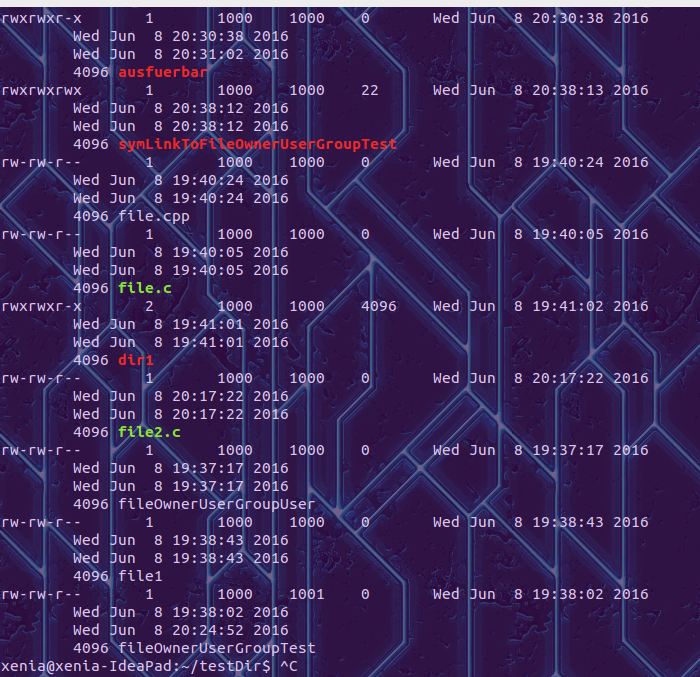
\includegraphics[width=200px, height = 200px]{image/ausgabe-l}

Nächste Test Parameter -g (kein owner id):
\begin{lstlisting}
~$	./myls -g
\end{lstlisting}
Wir sehen deutlich beim File fileOwnerUserGroupTest kein owner id(1000) angezeigt wird

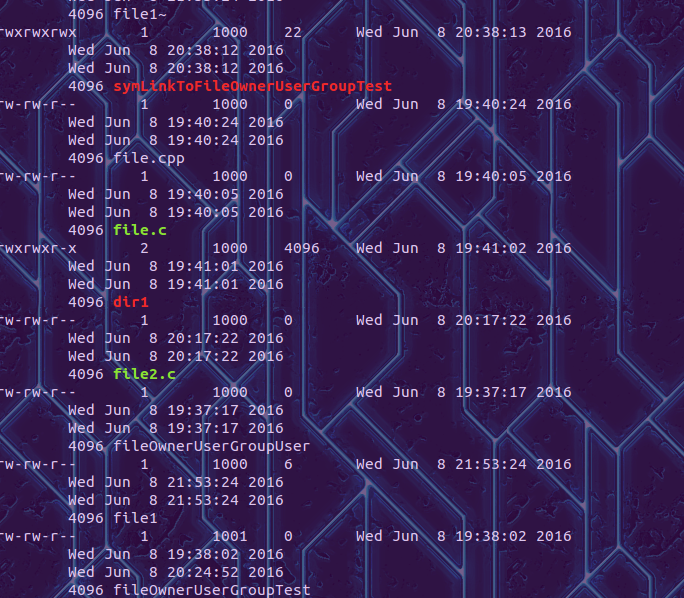
\includegraphics[width=200px, height = 200px]{image/ausgabe-g}

Nächste Test Parameter -g (kein group id):
\begin{lstlisting}
~$	./myls -o
\end{lstlisting}
Wir sehen deutlich beim File fileOwnerUserGroupTest kein group id(1001) angezeigt wird

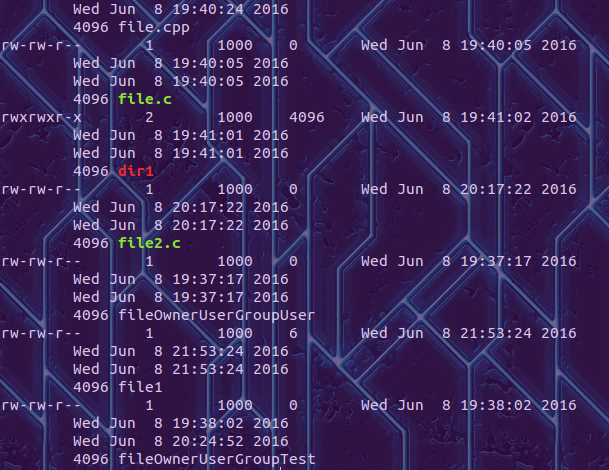
\includegraphics[width=200px, height = 200px]{image/ausgabe-o}

als nächstes testen wir alle Parameter -algo:
\begin{lstlisting}
~$	./myls -algo
\end{lstlisting}
hier wird weder owner id noch group id angezeigt

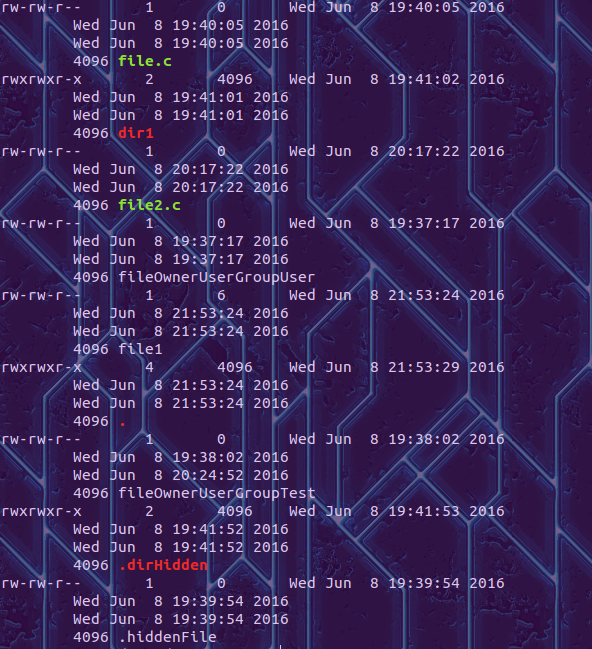
\includegraphics[width=200px, height = 200px]{image/ausgabe-algo}

und alle Parameter in beliebige  Reihenfolge:
\begin{lstlisting}
~$	./myls -oag
\end{lstlisting}

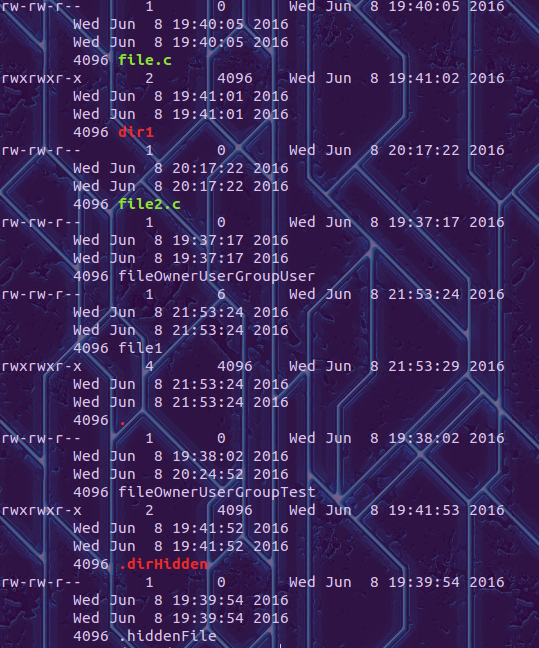
\includegraphics[width=200px, height = 200px]{image/ausgabe-oag}
